
To train the reinforcement learning policy for the agent, was adopted a tabular Q-learning approach. Multiple hyperparameter combinations were tested evaluating their performance through the cumulative reward across episodes and comparing athlete-specific training results.

\subsection{First Experiment: 500 Episodes}
In the initial experiment, training was limited to 500 episodes per combination (reported in table \ref{tab:hyperparameters-500}). This number was chosen to keep training time feasible while still allowing the Q-values to begin stabilizing and reveal early trends in learning performance.

\begin{table}[h!]
  \centering
  \begin{tabular}{l c c c c c}
    \toprule
    \textbf{Config Label} & $\alpha$ & $\gamma$ & $\epsilon_0$ & $\epsilon_{\min}$ & \textbf{decay} \\
    \midrule
    a10\_g95\_e20  & 0.10 & 0.95 & 0.20 & 0.01 & 0.99  \\
    a5\_g95\_e30   & 0.05 & 0.95 & 0.30 & 0.01 & 0.995 \\
    a10\_g99\_e20  & 0.10 & 0.99 & 0.20 & 0.01 & 0.98  \\
    a1\_g95\_e20   & 0.01 & 0.95 & 0.20 & 0.01 & 0.99  \\
    a10\_g90\_e20  & 0.10 & 0.90 & 0.20 & 0.01 & 0.98  \\
    a10\_g95\_e40  & 0.10 & 0.95 & 0.40 & 0.01 & 0.97  \\
    a5\_g99\_e30   & 0.05 & 0.99 & 0.30 & 0.01 & 0.995 \\
    a5\_g90\_e10   & 0.05 & 0.90 & 0.10 & 0.01 & 0.98  \\
    \bottomrule
  \end{tabular}
  \caption{Hyperparameter sets for 500-episode experiments}
  \label{tab:hp-500}
\end{table}


Each configuration was evaluated across the four predefined workouts and the three athlete profiles explained in section \ref{sec:settings}. For each of them was obtained a heatmap of the total rewards (fig. \ref{fig:amateur-500}, \ref{fig:runner-500}, \ref{fig:elite-500} ), representing the agent's performance across the different hyperparameter settings. 
In order to choose the best option, also the convergence of the Q-values was analyzed, which is shown in figures \ref{fig:convergence-500}. The convergence plots show how the Q-values stabilize over time, indicating that the agent is learning effectively.
\begin{figure}[!htbp]
    \centering
    \begin{subfigure}[t]{0.90\textwidth}
        \centering
        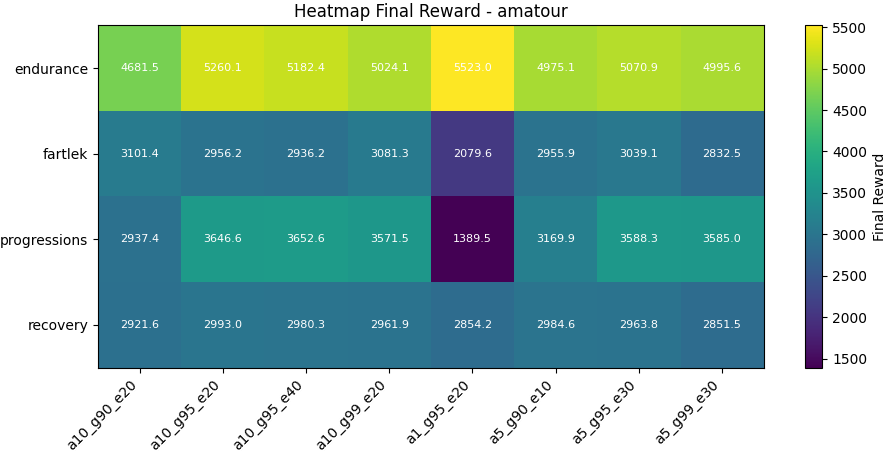
\includegraphics[width=\textwidth]{images/heatmap_final_amatour_500.png}
      \caption{Heatmap for the \textit{amateur} profile after 500 episodes}
    \label{fig:amateur-500}
    \end{subfigure}
    \begin{subfigure}[t]{0.90\textwidth}
        \centering
        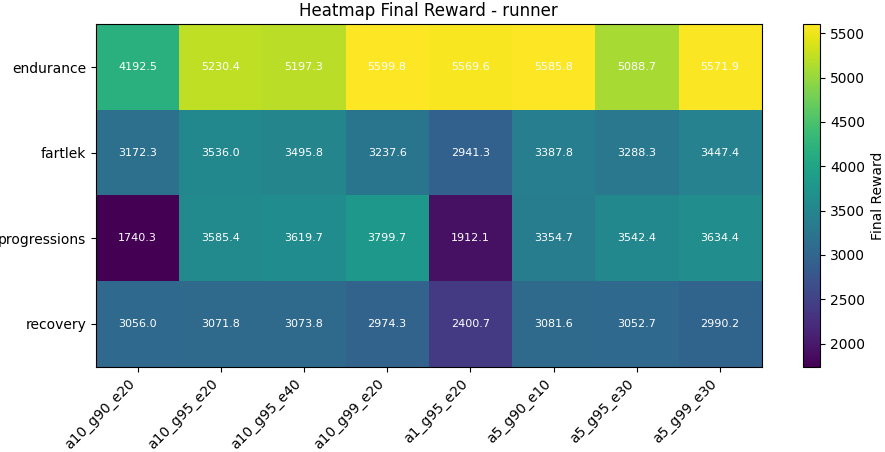
\includegraphics[width=\textwidth]{images/heatmap_final_runner_500.png}
        \caption{Heatmap for the \textit{runner} profile after 500 episodes}
    \label{fig:runner-500}
    \end{subfigure}
    \begin{subfigure}[t]{0.90\textwidth}
        \centering
        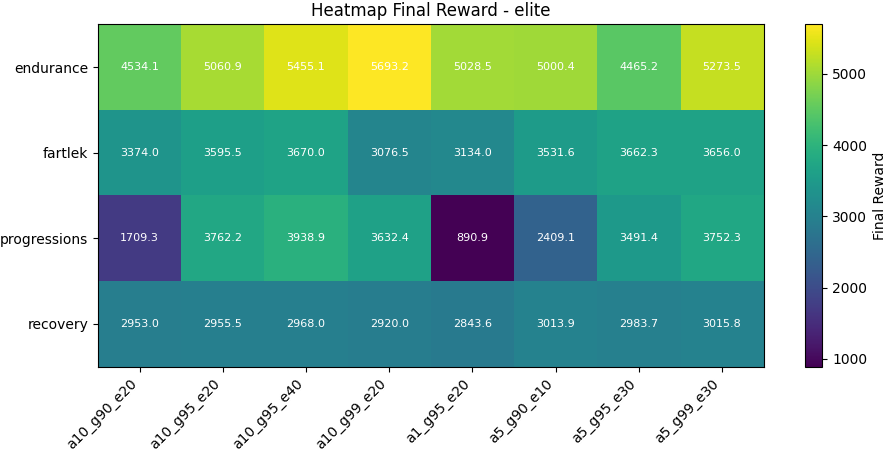
\includegraphics[width=\textwidth]{images/heatmap_final_elite_500.png}
        \caption{Heatmap for the \textit{elite} profile after 500 episodes}
    \label{fig:elite-500}
    \end{subfigure}
    \caption{Heatmaps of total rewards for different athlete profiles after 500 episodes}
\end{figure}

\begin{figure}[!htbp]
    \centering
    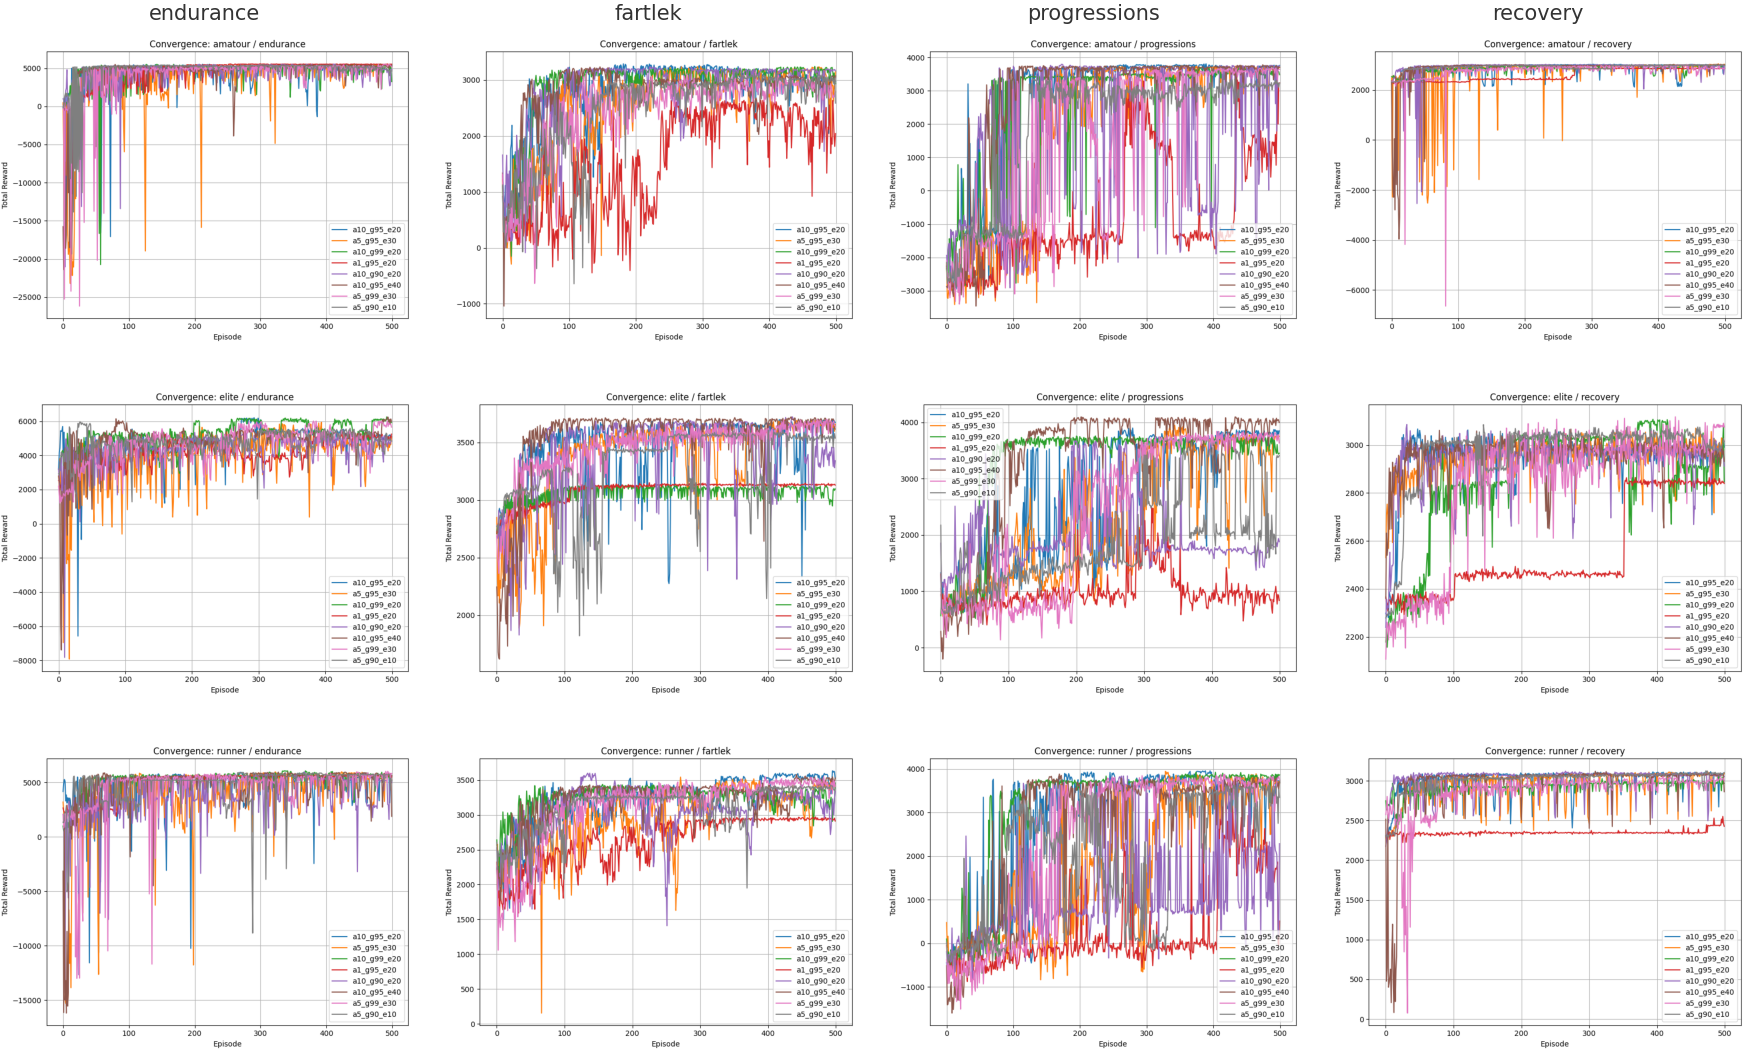
\includegraphics[width=1\textwidth]{images/convergence_grid_500_custom.png}
    \caption{Convergence of Q-values for tested hyperparameter configurations after 500 episodes.}
    \label{fig:convergence-500}
\end{figure}


Table~\ref{tab:hp-500} shows that most settings achieve a stable plateau well before the 500-episode mark; however, overly aggressive ``future-looking'' combinations (e.g., $\gamma = 0.99$) or highly exploratory starts (e.g., $\epsilon = 0.40$) sometimes dip late in noisy workouts like Fartlek and Progressions. The heatmaps in Figures~\ref{fig:amateur-500}--\ref{fig:elite-500} make it clear that \texttt{a10\_g95\_e20} consistently delivers the highest final rewards across all athlete types. For an \textit{elite} runner, who physiologically can sustain high intensity with minimal fatigue, that configuration tops the Endurance cell at about 5500 total reward, while still keeping fatigue low in recovery phases.

In contrast, an \textit{amateur} is expected to accumulate fatigue almost everywhere; indeed, only \texttt{a10\_g95\_e20} pushes them into medium fatigue zones without driving them into unsustainable high-fatigue levels. Less balanced choices either converge more slowly or produce erratic fatigue spikes, making them less reliable for a real-time pacing assistant.

\subsection{Second Experiment: 1000 Episodes}

To validate the consistency of the best configurations, or confirm that \texttt{a10\_g95\_e20} is the best combination, a reduced subset of hyperparameter combinations (based on the first test results) was run with 1000 episodes. 
This longer training period allowed more stable policy convergence and finer reward differentiation. 
Even if most of the convergence of the Q-values was already nearly reached, with 1000 episodes the agent was able to explore the state-action space further and refine its policy. 
The values of the hyperparameters used in this second experiment are shown in Table~\ref{tab:hp-1000}.

\begin{table}[h!]
  \centering
  \begin{tabular}{l c c c c c}
    \toprule
    \textbf{Config Label} & $\alpha$ & $\gamma$ & $\epsilon_0$ & $\epsilon_{\min}$ & \textbf{decay} \\
    \midrule
    a5\_g90\_e10   & 0.05 & 0.90 & 0.10 & 0.01 & 0.98  \\
    a10\_g95\_e20  & 0.10 & 0.95 & 0.20 & 0.01 & 0.99  \\
    a10\_g99\_e20  & 0.10 & 0.99 & 0.20 & 0.01 & 0.98  \\
    a5\_g95\_e30   & 0.05 & 0.95 & 0.30 & 0.01 & 0.995 \\
    \bottomrule
  \end{tabular}
  \caption{Hyperparameter sets for 1000-episode experiments}
  \label{tab:hp-1000}
\end{table}

\begin{figure}
    \centering
    \begin{subfigure}[t]{0.32\textwidth}
        \centering
        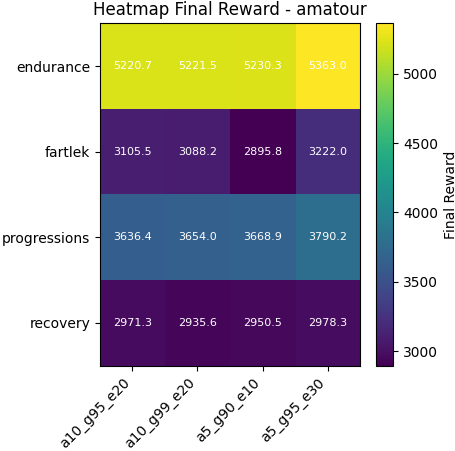
\includegraphics[width=\textwidth]{images/heatmap_final_amatour_1000.png}
      \caption{\textit{amateur} profile }
    \label{fig:amateur-1000}
    \end{subfigure}
    \begin{subfigure}[t]{0.32\textwidth}
        \centering
        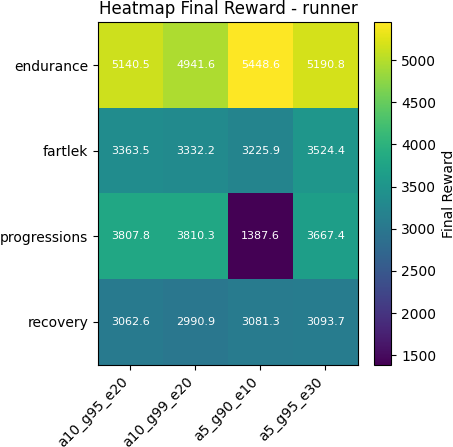
\includegraphics[width=\textwidth]{images/heatmap_final_runner_1000.png}
        \caption{\textit{runner} profile }
    \label{fig:runner-1000}
    \end{subfigure}
    \begin{subfigure}[t]{0.32\textwidth}
        \centering
        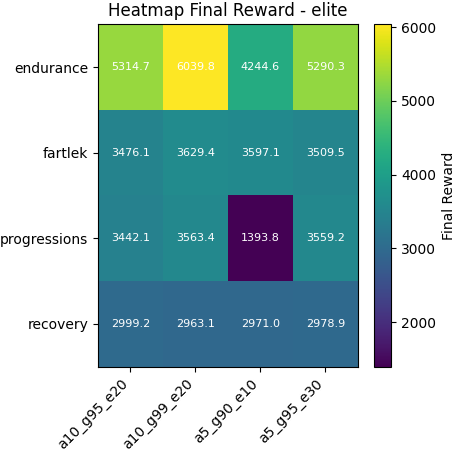
\includegraphics[width=\textwidth]{images/heatmap_final_elite_1000.png}
        \caption{\textit{elite} profile }
    \label{fig:elite-1000}
    \end{subfigure}
    \caption{Heatmaps of total rewards for different athlete profiles after 1000 episodes}
\end{figure}

\begin{figure}[t]
    \centering
    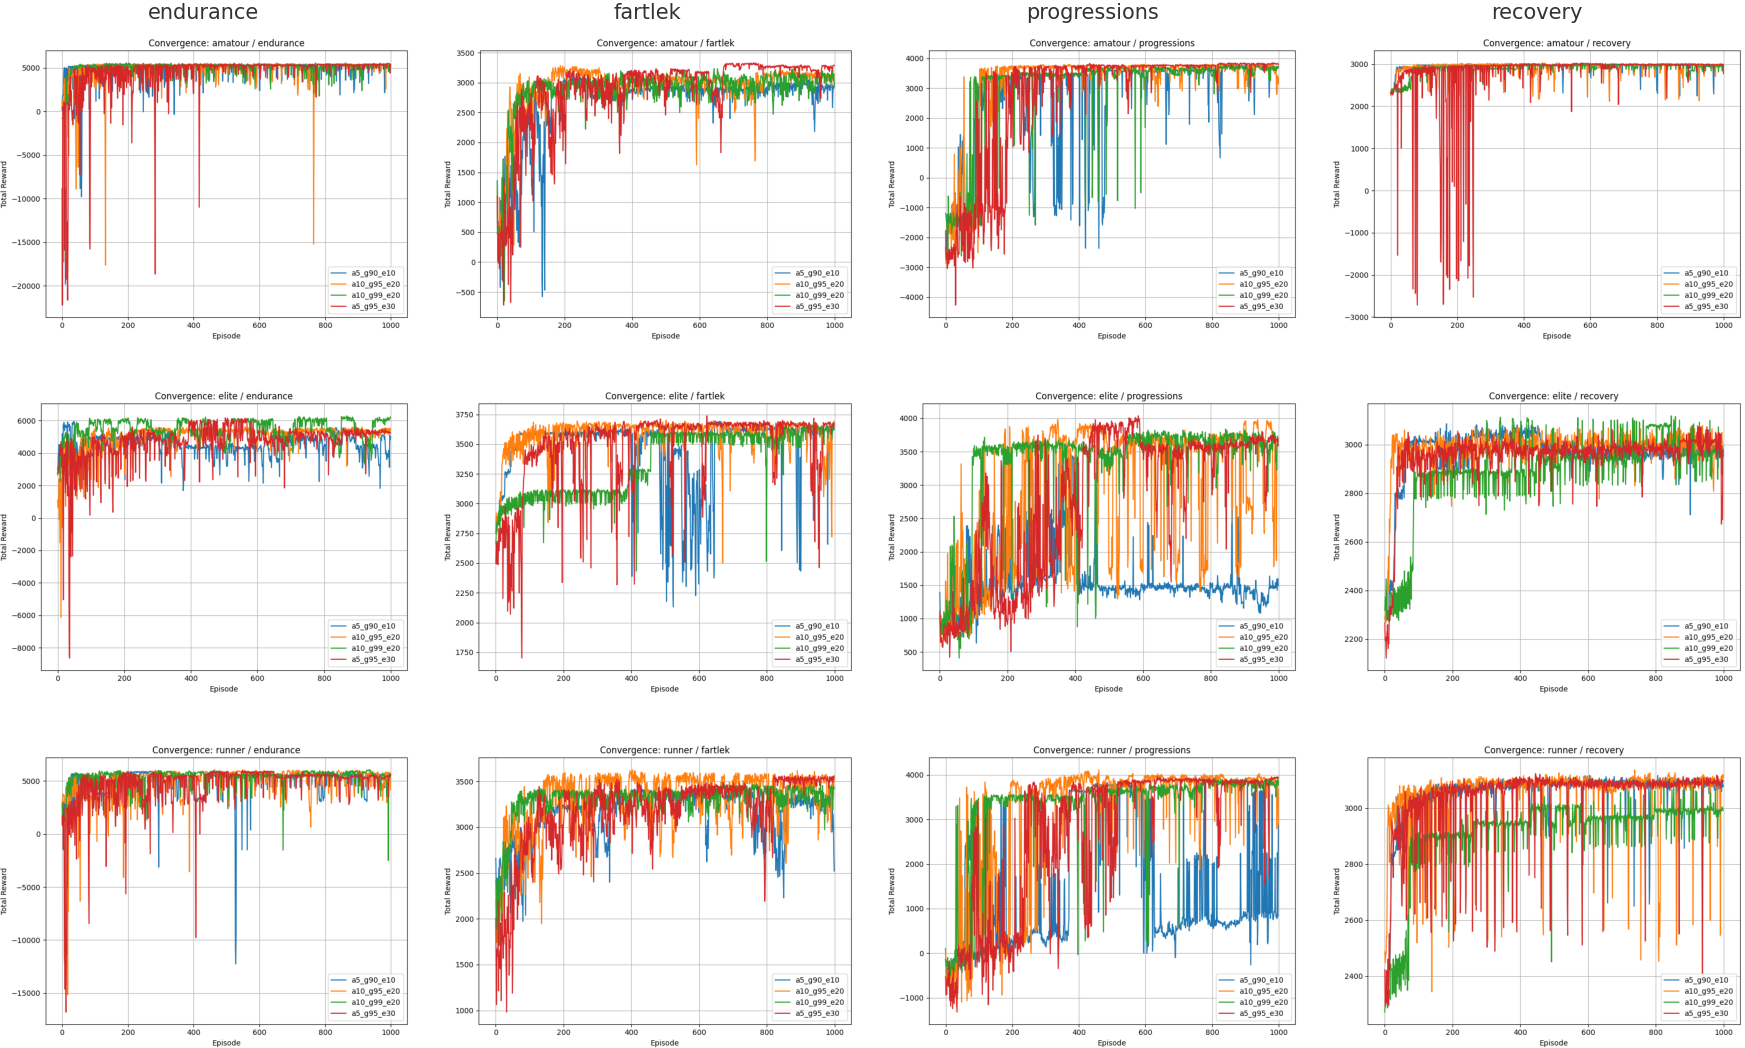
\includegraphics[width=0.99\textwidth]{images/convergence_grid_1000_custom.png}
    \caption{Convergence of Q-values for tested hyperparameter configurations after 1000 episodes.}
    \label{fig:convergence-1000}
\end{figure}

As shown in Figure~\ref{fig:convergence-1000}, all configurations now achieve very smooth, late-episode plateaus, with only minor oscillations remaining in the more complex workouts (\textit{fartlek}, \textit{progressions}). The heatmaps in Figures~\ref{fig:amateur-1000}~to~\ref{fig:elite-1000} reveal that \texttt{a10\_g95\_e20} not only retains its lead but widens the gap: it delivers the highest total reward for every athlete profile. From a physiological standpoint, our \textit{elite} runners benefit most from the balanced focus on immediate and future rewards, achieving peak performance in \textit{endurance} without unnecessary fatigue spikes in recovery. Conversely, \textit{amateurs}, who naturally accumulate fatigue more quickly, see a gentler fatigue profile under this configuration, avoiding severe high-fatigue states even in the toughest segments. The extended training thus confirms \texttt{a10\_g95\_e20} as the most robust and physiologically coherent choice across all scenarios.

\section{Final Q-tables and Policies}
After choosing the best hyperparameters (\texttt{alpha=0.1, gamma=0.95, epsilon=0.2}), a final run with 2000 episodes was performed to ensure the Q-values were fully converged and stable. This final run allowed the agent to refine its policy further, ensuring that it could make optimal decisions during each training session.
Different athletes, in the end, respond to the same training program in different ways, adapting their pace and heart rate according to their physiological parameters. The agent is able to adapt its behaviour to the athlete's profile, ensuring that the training is tailored to the athlete's needs.
A demonstration of the agent's performance can be seen in the video folder (and also in the figures below \ref{fig:video-amator}, \ref{fig:video-runner}, \ref{fig:video-elite}  ), where the agent is shown running in all possible combinations of \texttt{athlete}, \texttt{training program}, and also \texttt{different track} and below there 

\begin{figure}[h!]
    \centering
    \begin{subfigure}[t]{0.31\textwidth}
        \centering
        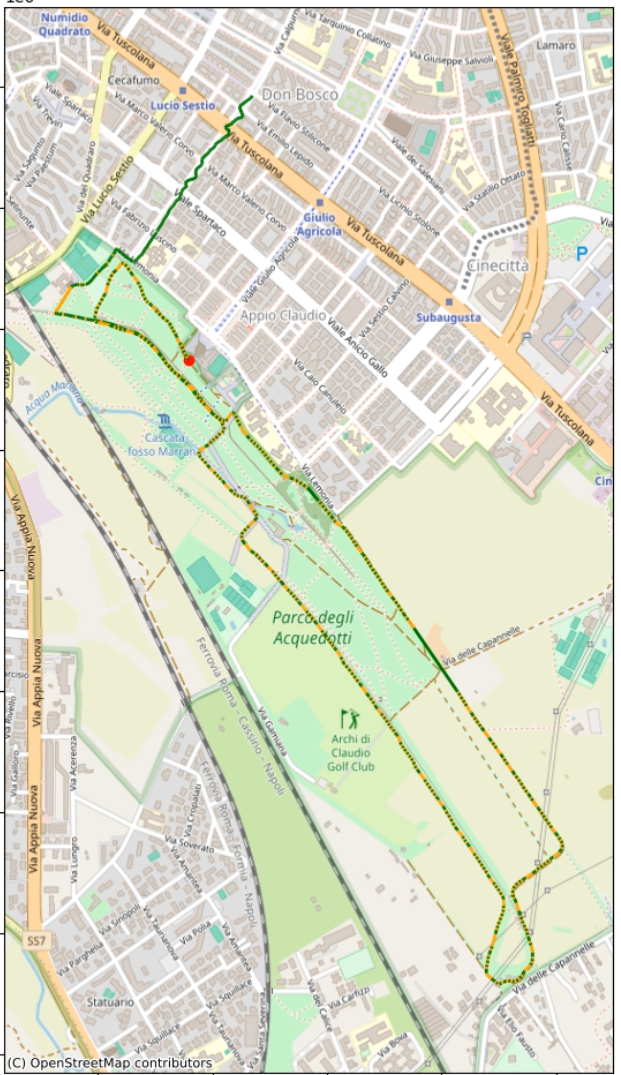
\includegraphics[width=\textwidth]{images/amatour-roma.png}
      \caption{\textit{amateur} simulation at Parco degli Acquedotti, Rome}
    \label{fig:video-amator}
    \end{subfigure}
    \begin{subfigure}[t]{0.305\textwidth}
        \centering
        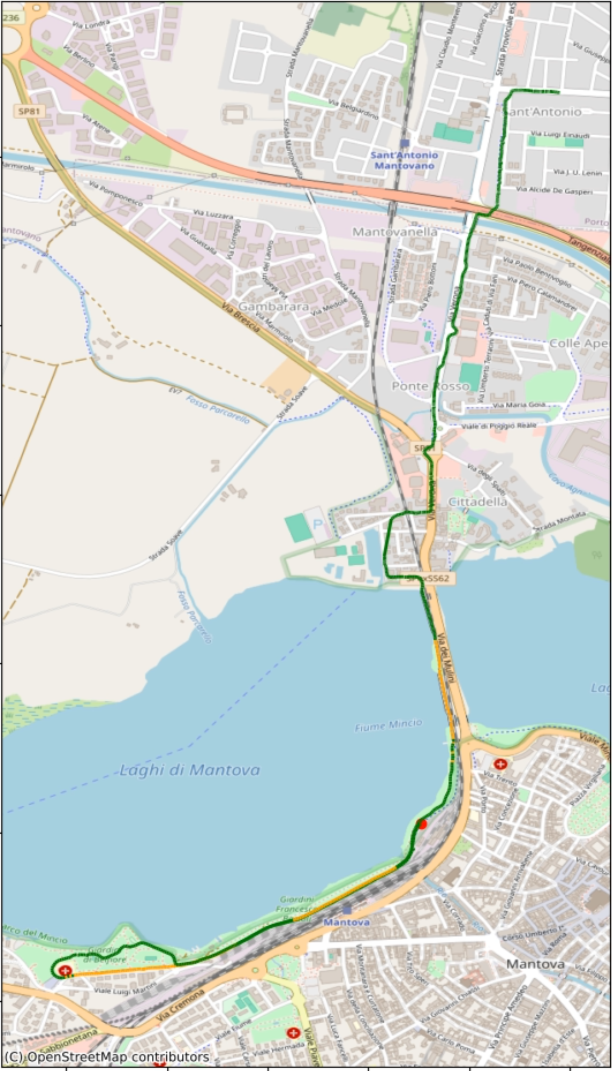
\includegraphics[width=\textwidth]{images/runner-belfiore.png}
        \caption{\textit{runner} simulation at Parco Belfiore, Mantova of a progression training program}
    \label{fig:video-runner}
    \end{subfigure}
    \begin{subfigure}[t]{0.31\textwidth}
        \centering
        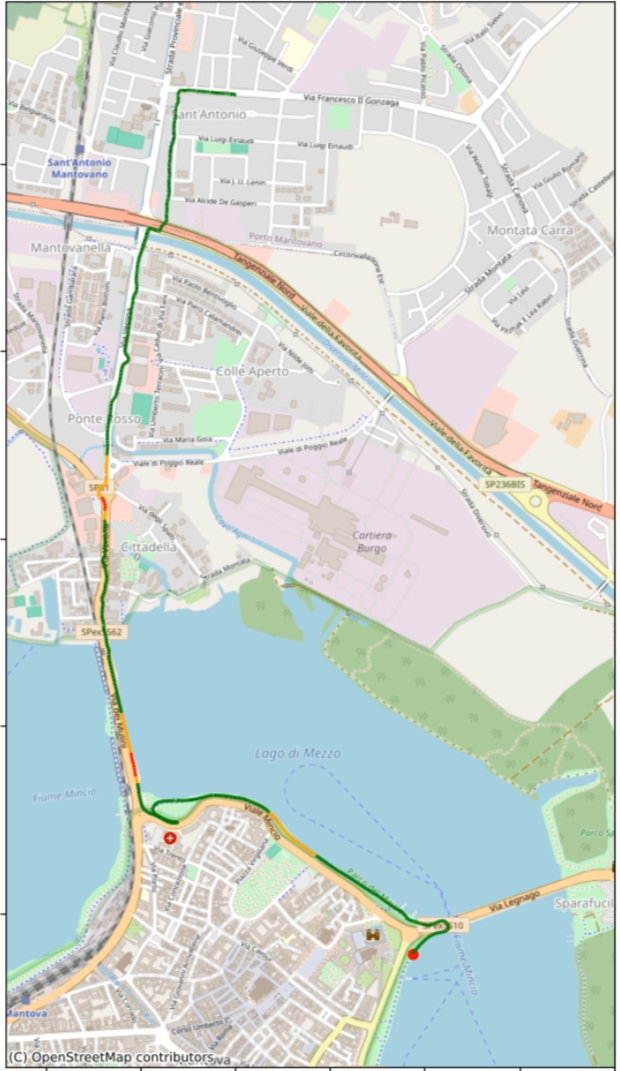
\includegraphics[width=\textwidth]{images/elite-fartlek.png}
        \caption{\textit{elite} simulation of the fartlek training program at Mantova, between the three lakes}
    \label{fig:video-elite}
    \end{subfigure}
    \caption{Screenshots from video simulations of the agent's performance across different athlete profiles and training programs. Red lines means high fatigue, yellow means medium fatigue, and green means low fatigue}
\end{figure}
